%%%%%%%%%%%%%%%%%%%%%%%%%%%%%%%%%%%%%%%%%%%%%%%%%%%%%%%%%%%%%%%%%%%%%%
% 
% 	Template for Producing ASP-DAC 2018 Proceedings
% 
%%%%%%%%%%%%%%%%%%%%%%%%%%%%%%%%%%%%%%%%%%%%%%%%%%%%%%%%%%%%%%%%%%%%%%
% History
% ??/??/?? Designed by Hiroaki Kunieda (ASP-DAC '97 Publication Chair)
% 09/22/97 Modified and small bug fixed by Masaharu Imai 
% 	   (ASP-DAC '98 Publication Chair)
% 11/02/98 Modified by Tsuyoshi Isshiki
% 	   (ASP-DAC 2000 TPS Secretary)
% 7/24/00 Modified by Kiyoharu Hamaguchi
% 	   (ASP-DAC 2001 Publication chair)
% 6/18/02 Modified by Kazutoshi Kobayashi
% 	   (ASP-DAC 2003 Publication Co-Chair)
% 5/27/03 Modified by Kiyoharu Hamaguchi
% 	   (ASP-DAC 2004 TPC secretary)
% 6/10/03 Modified by Kazutoshi Kobayashi for Latex2e
% 	   (ASP-DAC 2004 Publication Co-Chair)
% 6/01/05 Modified by Nozomu Togawa
% 	   (ASP-DAC 2006 Publication Chair)
% 6/01/06 Modified by Hiroyuki Ochi
% 	   (ASP-DAC 2007 Publication Chair)
% 5/30/08 Modified by Nozomu Togawa
% 	   (ASP-DAC 2009 Publication Co-Chair)
% 4/30/10 Modified by Masashi Imai
% 	   (ASP-DAC 2011 Publication Chair)
% 3/20/12 Modified by Masashi Imai
% 	   (ASP-DAC 2013 Publication Chair)
% 5/01/14 Modified by Masashi Imai
% 	   (ASP-DAC 2015 Publication Chair)
% 4/24/16 Modified by Masashi Imai
% 	   (ASP-DAC 2017 Publication Chair)
% 2/06/17 Modified by Jongeun Lee
% 	   (ASP-DAC 2018 Publication Chair)
%%%%%%%%%%%%%%%%%%%%%%%%%%%%%%%%%%%%%%%%%%%%%%%%%%%%%%%%%%%%%%%%%%%%%%
% If you have any problem, please contact ASP-DAC 2018 Publication
% Chair by E-mail at "jlee@unist.ac.kr.''
%%%%%%%%%%%%%%%%%%%%%%%%%%%%%%%%%%%%%%%%%%%%%%%%%%%%%%%%%%%%%%%%%%%%%%
%
\documentclass[twocolumn]{article}
%% If you use dvips and ps2pdf, please use Postscript font 
%% and uncomment the line below.
%%\usepackage{times}
\usepackage[dvipdfmx]{graphicx}
\usepackage{bm}
\pagestyle{empty}
%set paper size
%for A4 paper
\topmargin      29mm    %bottom margin 30mm
\oddsidemargin  15mm    %left & right margin 15mm

%for 8 1/2" x 11" paper paper, use the following definition
%\topmargin     17mm    %bottom margin 24mm
%\oddsidemargin 18mm    %left margin 18mm & right margin 17mm

%text sizes
\textwidth  180mm
\textheight 238mm
\columnsep  5.0mm
\parindent  3.5mm

%misc parameters
\headsep 0mm  \headheight 0mm
\footskip 18mm
%\footheight 6mm

%conversion to values for LaTeX
\advance\topmargin-1in\advance\oddsidemargin-1in
\evensidemargin\oddsidemargin

\makeatletter
%as Latex considers descenders in its calculation of interline spacing,
%to get 12 point spacing for normalsize text, must set it to 10 points
\def\@normalsize{\@setsize\normalsize{12pt}\xpt\@xpt
\abovedisplayskip 10pt plus2pt minus5pt\belowdisplayskip \abovedisplayskip
\abovedisplayshortskip \z@ plus3pt\belowdisplayshortskip 6pt plus3pt
minus3pt\let\@listi\@listI}

%interline spaceing and title font for section
\def\section{\@startsection {section}{1}{\z@}{20pt plus 2pt minus 2pt}
{8pt plus 2pt minus 2pt}{\centering\normalsize\sc
\edef\@svsec{\thesection.\ }}}
\def\thesection{\Roman{section}}

%interline spacing and title font for subsection
\def\subsection{\@startsection {subsection}{2}{\z@}{16pt plus 2pt minus 2pt}
{6pt plus 2pt minus 2pt}{\normalsize\sl
\edef\@svsec{\thesubsection.\ }}}
\def\thesubsection{\Alph{subsection}}

%figures/tables captions
\long\def\@makecaption#1#2{
\vskip10pt\begin{center} #1 #2 \end{center}\par\vskip 1pt}
\def\fnum@figure{\raggedright{\footnotesize Fig. \thefigure }.%
\footnotesize}
\def\fnum@table{\footnotesize TABLE \thetable\\\footnotesize\sc}
\def\thetable{\Roman{table}}

\makeatother

\renewcommand{\floatpagefraction}{0.99}

%%%%%%%%%%%%%%%%%%%%%%%%%%%%%%%%%%%%%%%%%%%%%%%%%%%%%%%%%%%%%%%%%%%%%%%

\begin{document}
%date not printed
\date{}

%make title
\title{\Large\textbf{A Deep Neural Network Based Approach to Aestheticize Schematics}}%\\~\\
%\large\textbf{
%Preparation of Papers in Two-Column Format\\
%for the ASP-DAC 2018 (\LaTeX2e version)}}	% Modified by K. Kobayashi 18/06/02

%for single author
%\author{Center the Authors Names Here \\
%Center the Affiliations Here\\
%Center the City, Stats and Country Here\\
%{\small (it is your option if you want your entire address listed)}}

%for two authors
\author{Author 1 and Author 2}
\maketitle
\thispagestyle{empty}

{\small\textbf{Abstract---
This paper proposes a novel method to combine schematic expression
and deep neural network to automatically aestheticize schematics.
Schematics are encoded to vectors so that the neural network can accept them.
Neural network is trained in supervised learning
with schematics and edit commands
which do not change the semantics of the schematics.
After training, schematics which are not a part of training data
are fed to trained neural network,
and the neural network makes given schematics aesthetic.
When trained with 33\% of all data,
the trained neural network has successfully aestheticized
95\% of schematics unused in traning.
}}

\section{Introduction}

Electronic design automation (EDA) has applied a positive feedback
for computer design by deploying computers themselves,
introducing an acceleration to growth of computing power
and achieving an exponential growth, along with Moore's law.
Increasing the transistor count,
functionality of electronic devices and their complexity of design,
EDA has supported the development, by means of circuit simulator,
logic synthesis, high-level synthesis, automatic layout,
design rule checker, kinds of equivalence checkers,
automatic test pattern generator (ATPG), etc.
Those EDA tools handle topology information expressed as text data
called netlist which is easy for computer to deal with.
As well, output data from EDA are also text-based netlist,
which are result of automatic layout, result of parasitic extraction, etc.
Those text-based data often have to be manually analyzed
for debug or engineering change order (ECO),
but the analysis is error prone.
Then schematics are often manually drawn down from netlist.
Electronic circuitry is designed on schematic,
especially for analogue circuit,
because schematics are more readable and understandable
than text-based netlist.
Even though digital circuit is often designed
on hardware description language (HDL),
schematics are useful for complex and clock-cycle-timing-critical design,
e.g., pipeline \cite{ph}.
So far, methods to automatically generate schematics from netlist or HDL
have been proposed
\cite{nauts}
\cite{anshul}
\cite{fiduccia}
\cite{chun}
\cite{green}
\cite{tsung}
\cite{bogdan}.

Each of them focuses only on one of analog circuit,
gate level netlist of digital circuit
or more higher level HDL visualization.
And the best shape of schematic is likely to depend on
type of circuit, each project, or each individual.
Recently, interest to machine learning is raining,
and some studies have applied machine-learning-based techniques
to unprecedented realm of EDA \cite{fan} \cite{sourav}.
Among machine learning techniques,
deep neural network has demonstrated great performance
in application of recognizing field data
expanded on 2-dimensional space,
e.g., bitmap image or board game field \cite{nips} \cite{alphago}.

This paper proposes a novel method to combine schematic expression
which is another 2-dimensional field data
and deep neural network to automatically manipulate schematics
and to achieve human-readable ones, based on its training result.
Schematics are encoded to vectors so that the neural network can accept them.
The encoded schematics and corresponding preferred schematic edit commands,
which are also encoded and do not change semantics of schematics,
are given as training data.
After training, schematics which are not a part of training data
are fed to trained neural network,
and the neural network makes given schematics aesthetic.

\section{Concept}

\begin{figure}[!tp]
 \begin{center}
  \begin{minipage}{\hsize}
   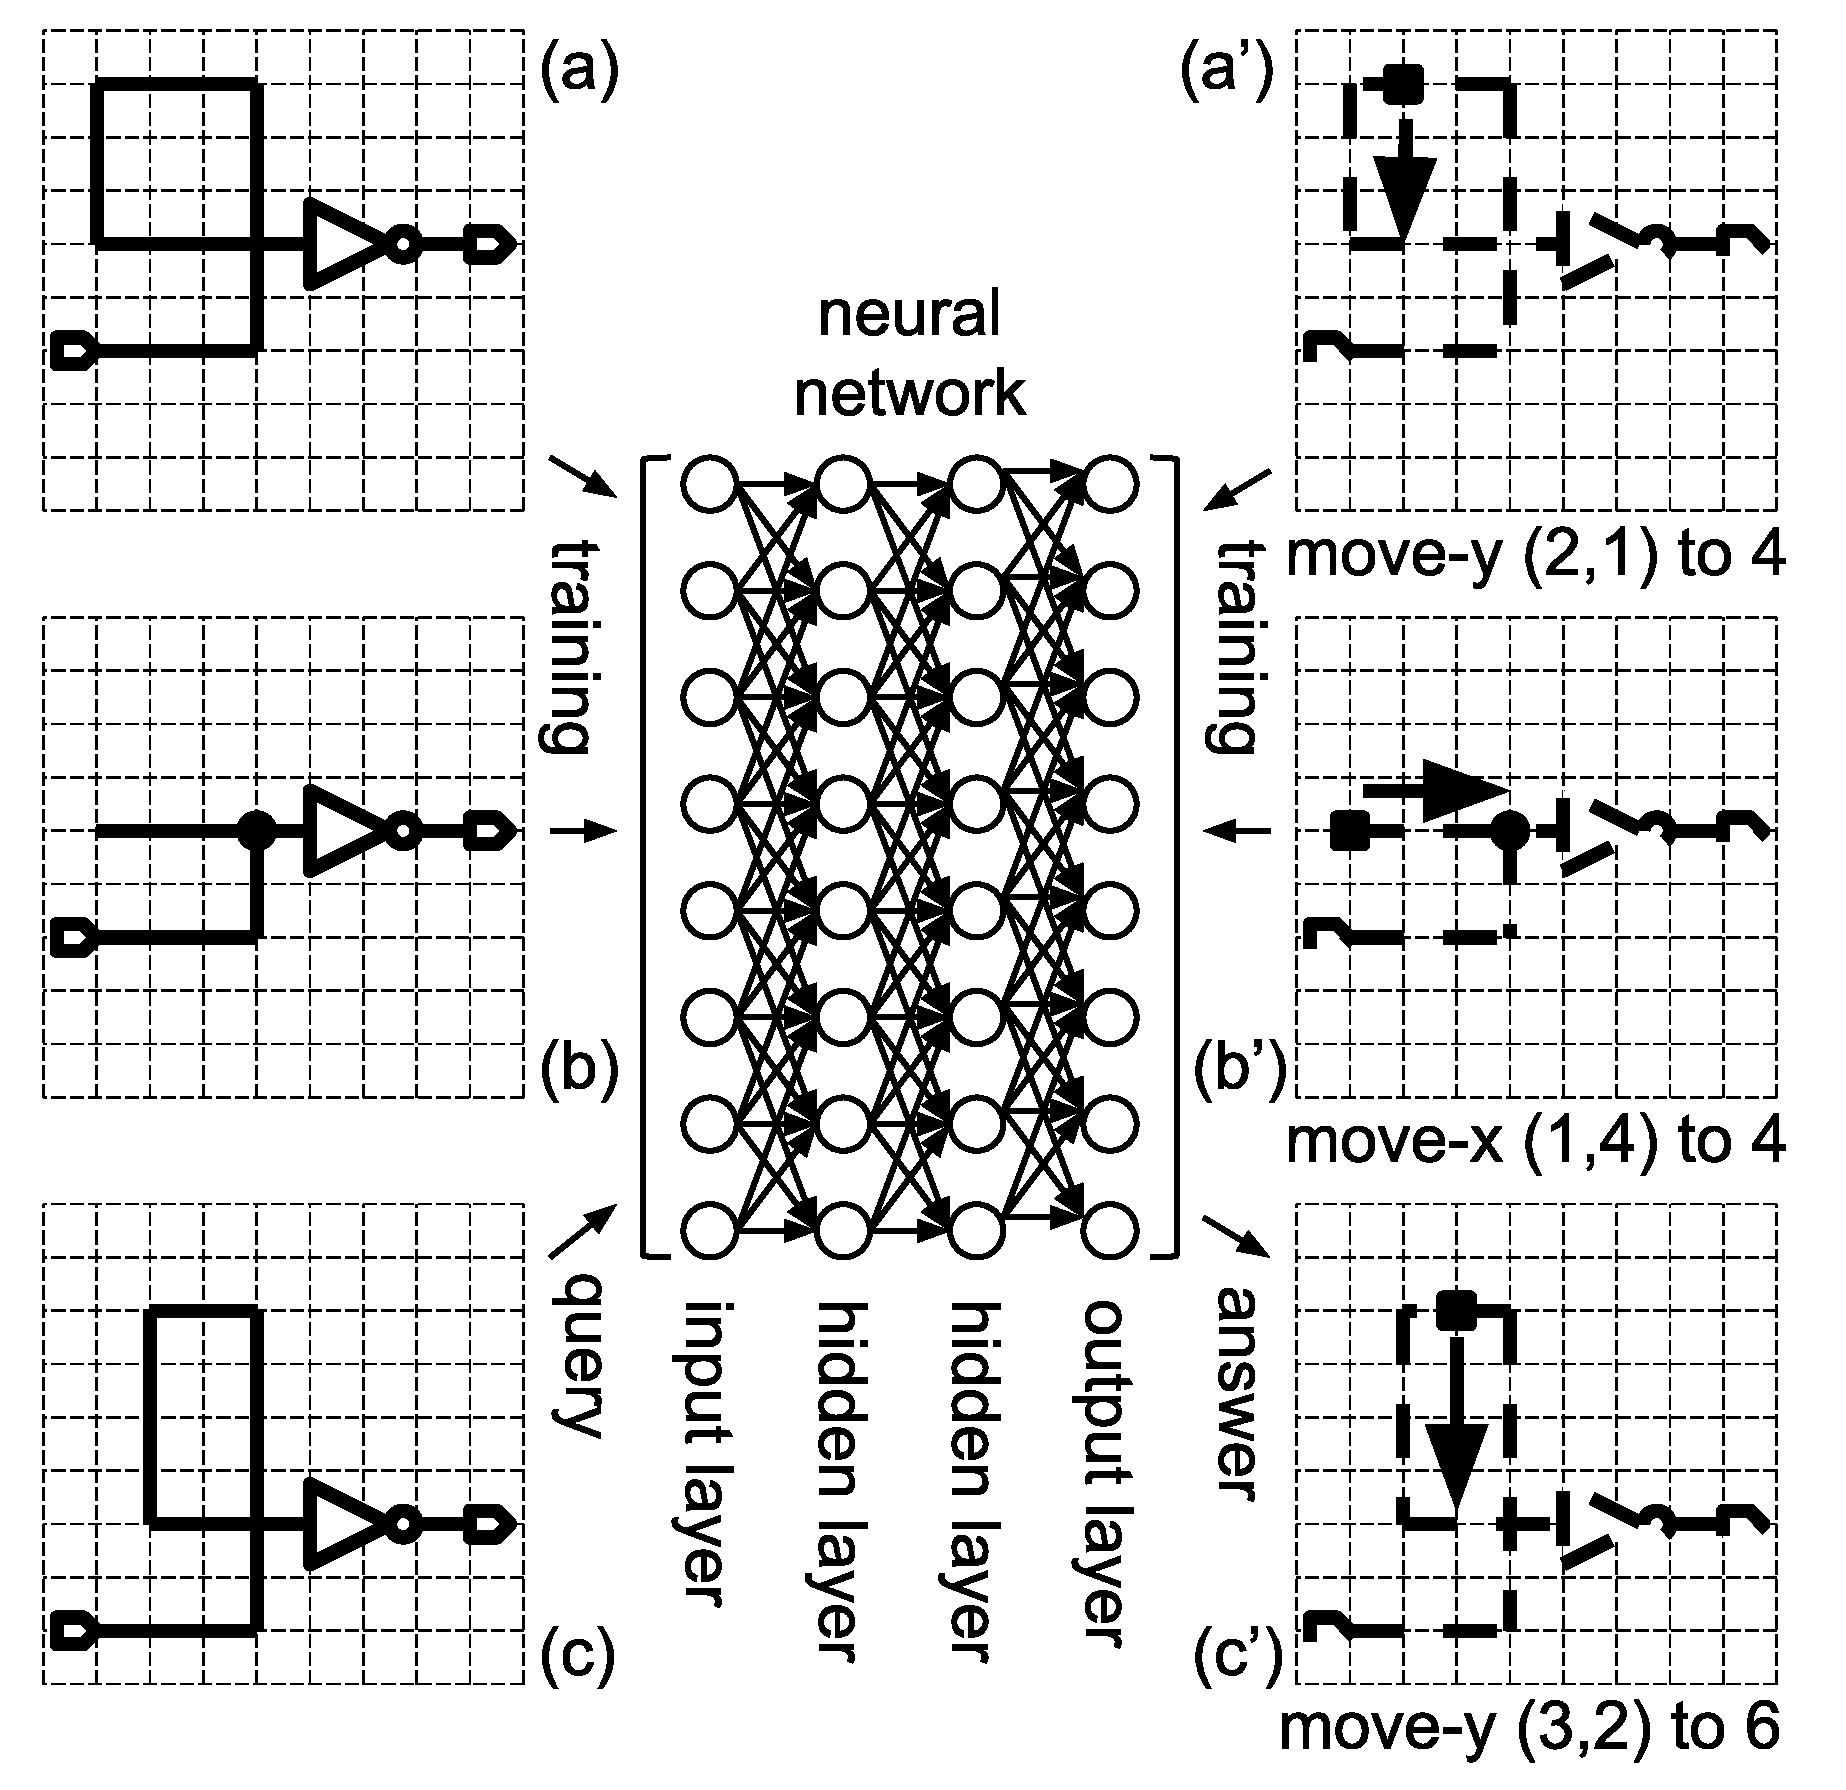
\includegraphics[width=\hsize]{fig/nn_schem_05.eps}
   \caption{Training and querying neural network.}
   \label{fig:nn_schem}
  \end{minipage}
 \end{center}
\end{figure}

This section describes how a neural network is
combined with schematic diagrams,
a basic concept of which is shown in Fig.\ \ref{fig:nn_schem}.
The neural network will aestheticize given schematics after training.

Training phase is shown in Fig.\ \ref{fig:nn_schem} (a), (a'), (b) and (b')
where pairs of a schematic diagram and a preferred edit command
to make it cleaner are given to the neural network.
The neural network updates its internal parameters as knowledge obtained
from the training.
Note that training data go into to output layer
as well as input layer in traning phase,
even though the layer is called {\it output layer}.
After training, the neural network generates schematic edit commands
from the output layer even for one the network has not experienced,
as shown in Fig.\ \ref{fig:nn_schem} (c) and (c').

\begin{figure}[!tb]
 \begin{center}
  \begin{minipage}{\hsize}
   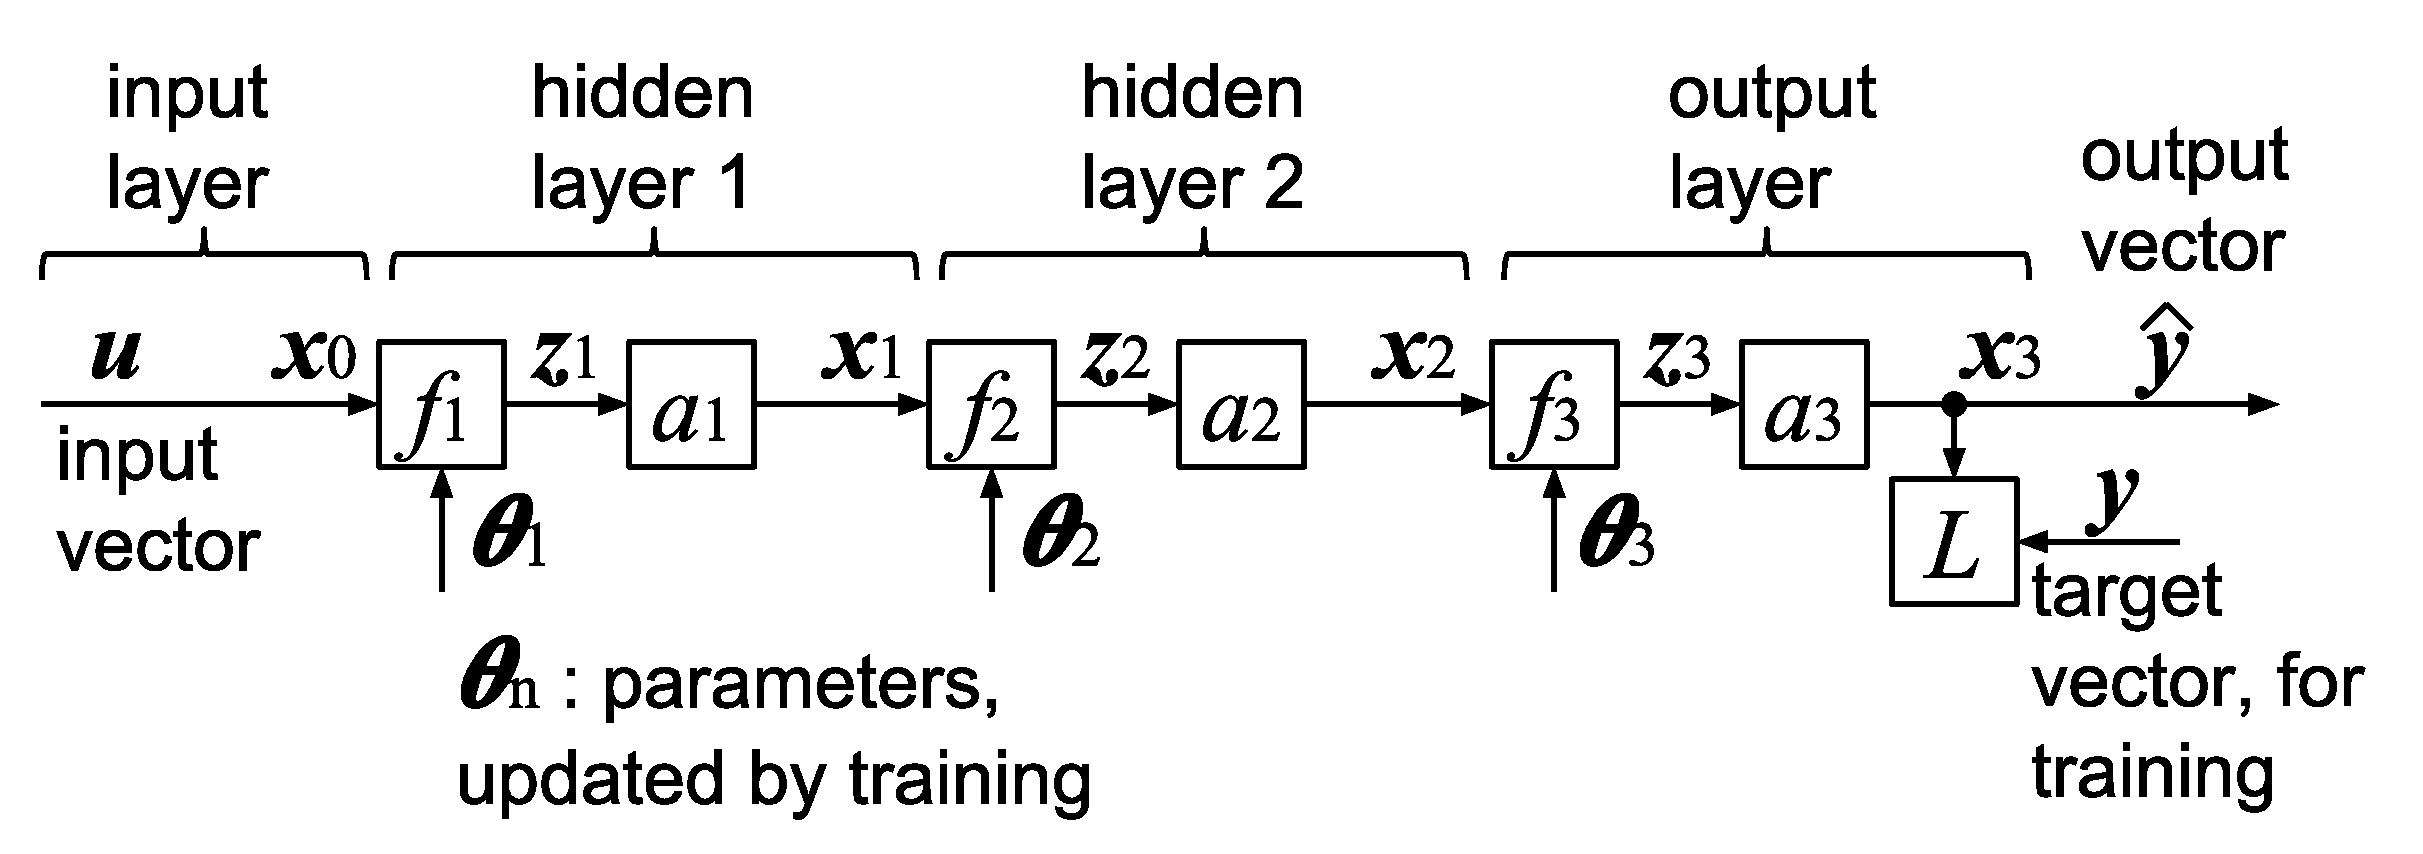
\includegraphics[width=\hsize]{fig/deep_feedforward_03.eps}
   \caption{A deep feedforward network.}
   \label{fig:deep_feedforward}
  \end{minipage}
 \end{center}
\end{figure}

An neural network architecture called {\it deep feedforward network} is used,
and it is trained by {\it stochastic gradient descent} (SGC)
as descripbed in \cite{mit}.
Figure \ref{fig:deep_feedforward} shows an example of deep feedforward network.
It consists of an input layer, some hidden layers and an output layer,
with no feedback path.
Based on trained parameters ${\bm \theta}_n$,
it generates an output vector denoted as $\hat{\bf y}$
which corresponds to preferred edit command for a given input vector
${\bf u}$ which is an encoded schematic diagram.
Formally, $\hat{\bf y}$ is calculated as;
\begin{eqnarray}
\hat{\bf y} &=& {\bf x}_N \\
{\bf x}_n &=& a_n({\bf z}_n) \\
{\bf z}_n &=& f_n({\bf x}_{n-1}, {\bm \theta}_n)\\
{\bf x}_0 &=& {\bf u}
\end{eqnarray}
where $N$ is the total number of hidden and output layers,
$n$ is an integer ranging from 1 to $N$.
$f_n$ is a weight function to weigh elements of layer input.
$a_n$ is an activation function,
typically clipping too large or too small output values of $f_n$.

As described below,
SGC updates ${\bm \theta}_n$ so that it reduces an error
between $\hat{\bf y}$ and ${\bf y}$,
where ${\bf y}$ is a target vector
which a neural network is trained to obtain
for an given input vector ${\bf u}$.
Given an loss function
$L(\hat{\bf y}({\bf u},{\bm \theta}_1,\cdots,{\bm \theta}_N),{\bf y})$
which evaluates the error between $\hat{\bf y}$ and ${\bf y}$,
${\bm \theta}_n$ is updated along with the gradient of $L$ as follows:
\begin{eqnarray}
{\bm \theta}_n \leftarrow
(1-\lambda){\bm \theta}_n
- \epsilon
  \frac{1}{M}\sum_{i=1}^M
  \frac{\partial L(\hat{\bf y}_i({\bf u}_i,{\bm \theta}_1,
                               \cdots,{\bm \theta}_N),
                   {\bf y}_i)}
       {\partial {\bm \theta}_n}\label{eqn:sgd}
\end{eqnarray}
where an input vector ${\bf u}_i$ is accompanied with a subscript $i$
to show that ${\bf u}_i$ is an array of vectors randomly picked up
from training data set.
$\hat{\bf y}_i$ and ${\bf y}_i$ are vector arrays there, too.
The number of vectors $M$ is called {\it minibatch size}.
$\lambda$ is weight decay to avoid overfitting,
$\epsilon$ is learning rate.
Values smaller than 1 and slightly more than 0 are chosen
for $\lambda$ and $\epsilon$.
By repeatedly applying the equation (\ref{eqn:sgd}),
the parameter ${\bm \theta}_n$ gets close to the optimal value.

\begin{figure}[!tp]
 \begin{center}
  \begin{minipage}{\hsize}
   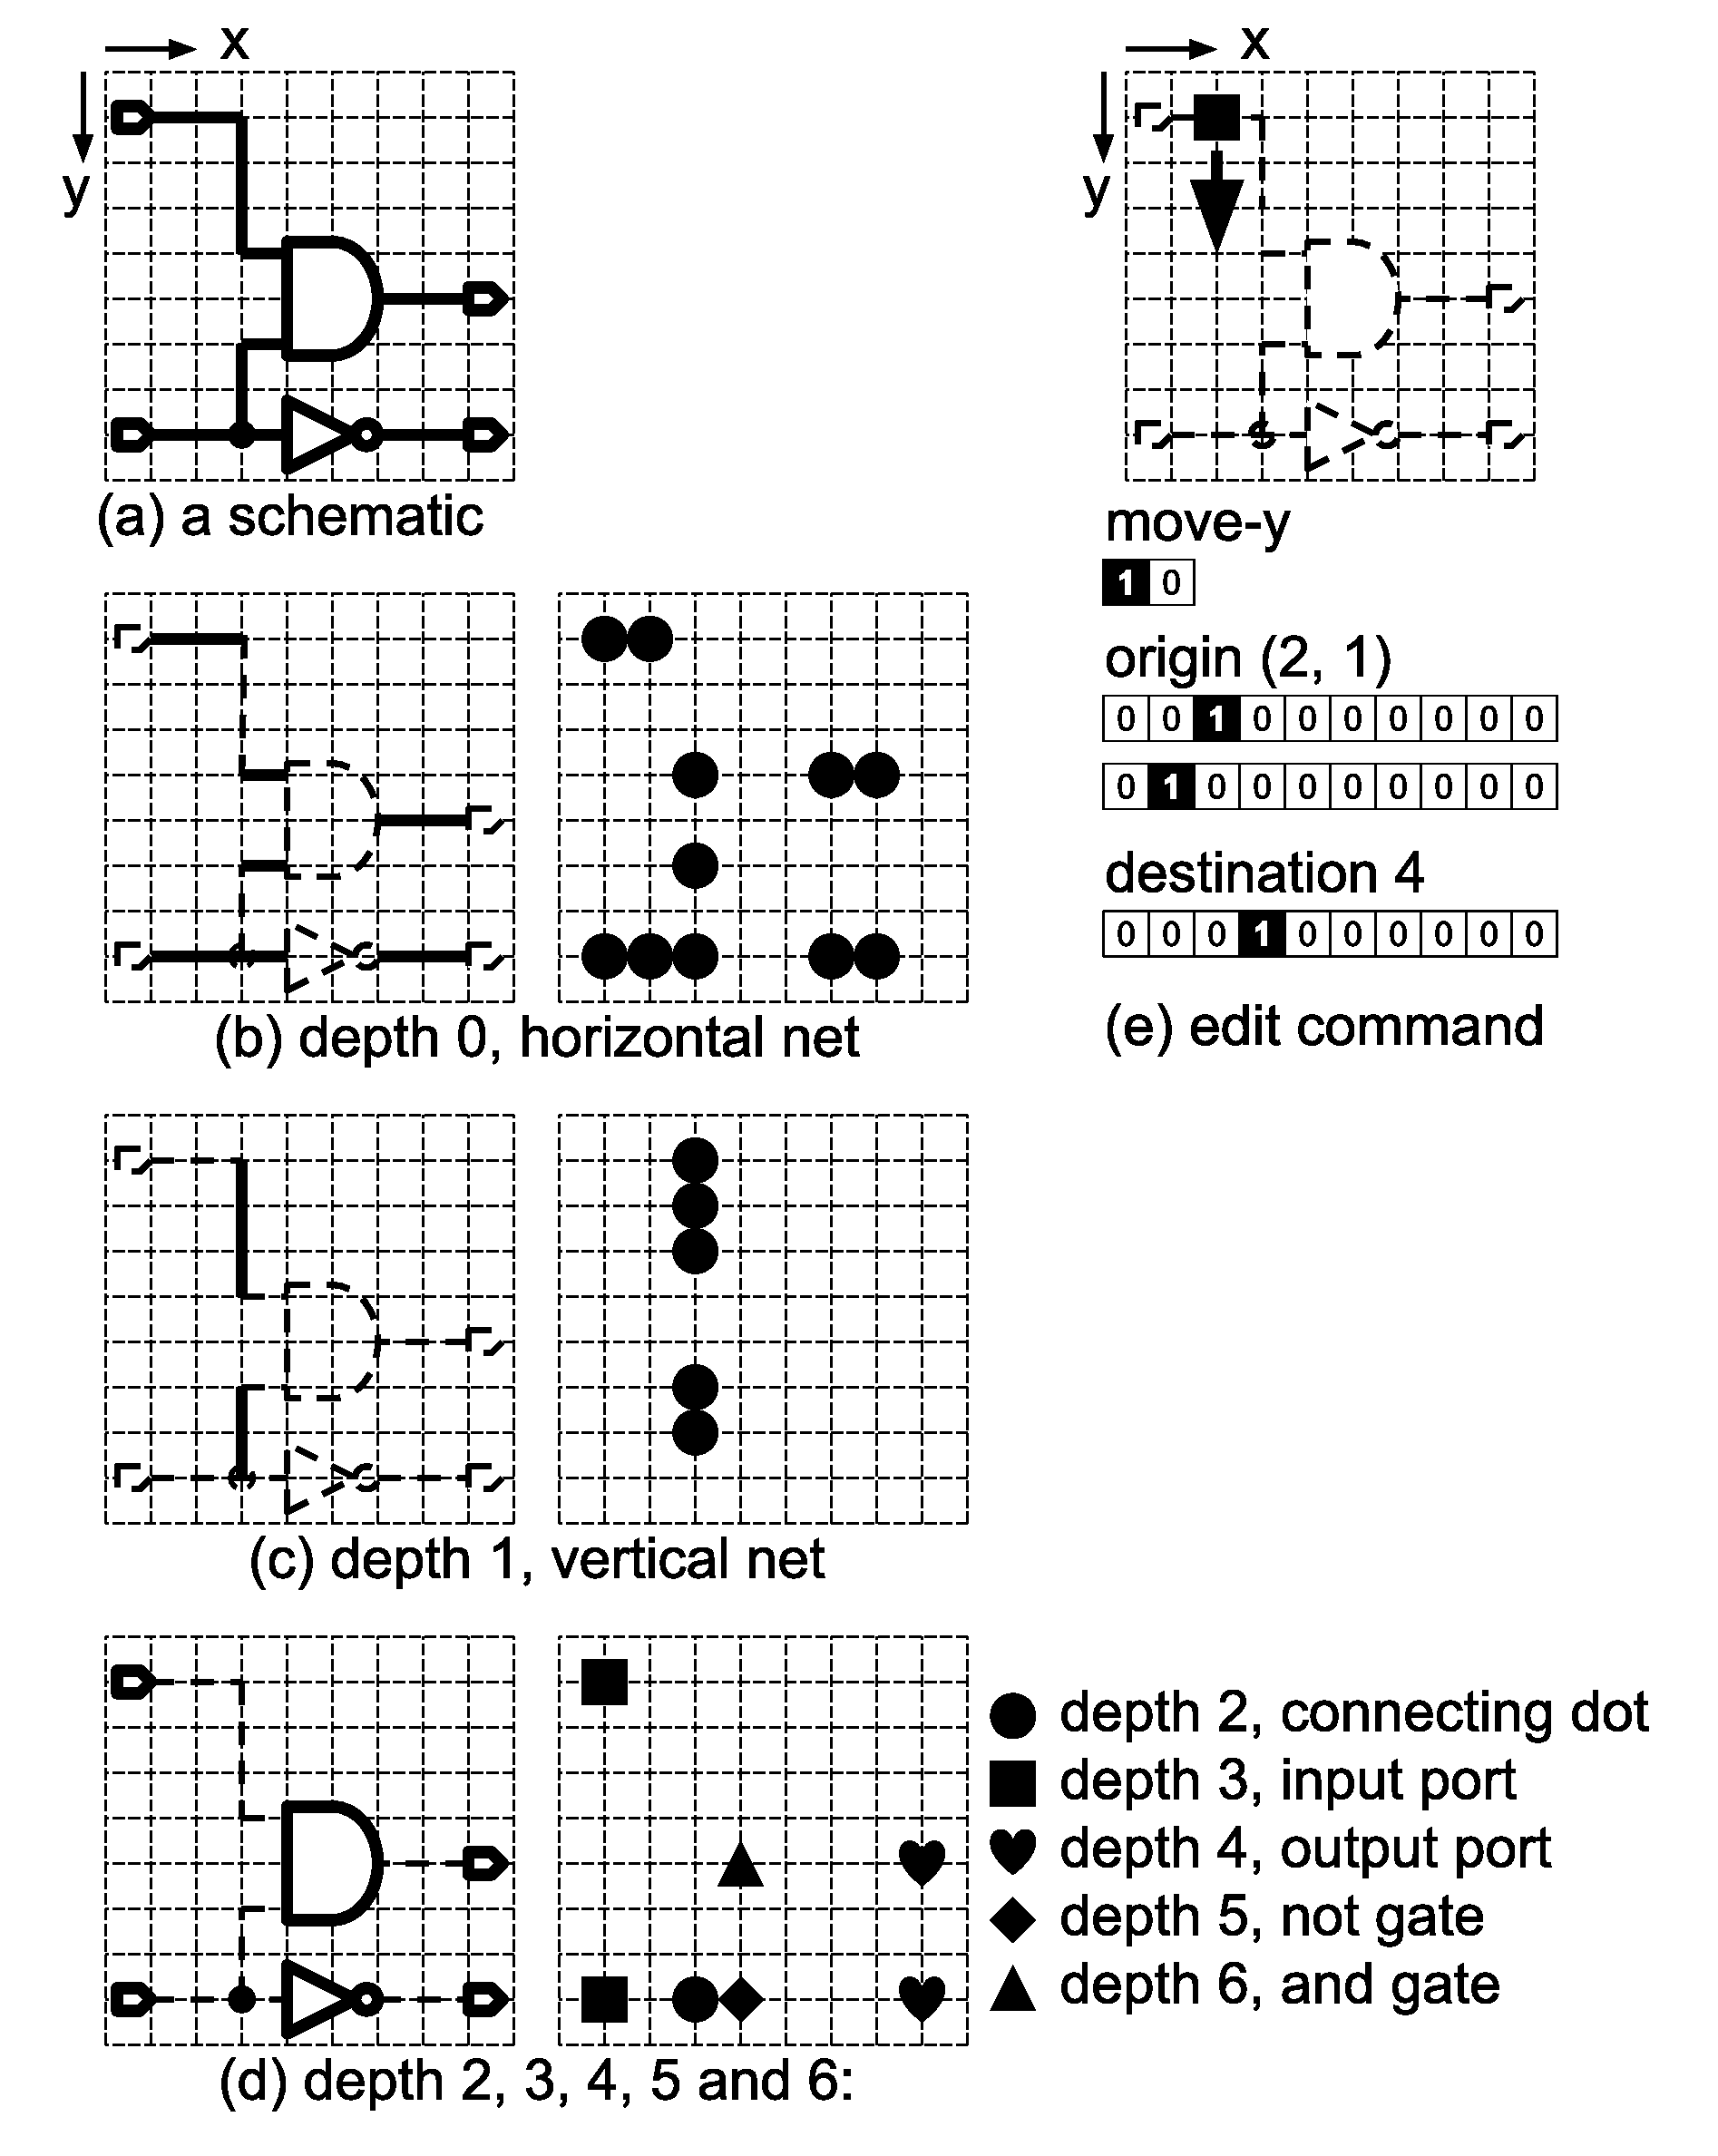
\includegraphics[width=\hsize]{fig/encode_02.eps}
   \caption{Schamatics and commands encoding.}
   \label{fig:encode}
  \end{minipage}
 \end{center}
\end{figure}

It is shown in Fig.\ \ref{fig:encode} how to encode
schematics and edit commands so that the neural network can accept them.
Figure \ref{fig:encode} (a) shows a schematic composed of
inputs ports, output ports, an and-gate, a not-gate,
horizontal nets, vertical nets, and a connecting dot.
Elements on a schematic diagram are
mapped onto 3-dimensional space.
Figure \ref{fig:encode} (b) picks up horizontal nets appearing
in Fig.\ \ref{fig:encode} (a), and they are mapped to depth 0.
The depth 0 is composed of a 2-dimensional matrix which size is the same
as that of a given schematic diagram.
On the right side of Fig.\ \ref{fig:encode} (b),
dots appear at coordinates where horizontal nets exist.
A dot is mapped to a value of 1.0.
Other points correnspond to 0.0.
As shown in Fig.\ \ref{fig:encode} (c),
vertical nets are mapped to depth 1.
As well, connecting dots, input ports, output ports, not-gates and and-gates
are mapped to depth 2, 3, 4, 5 and 6, respectively.

\begin{figure*}[!tp]
 \begin{center}
  \begin{minipage}{\hsize}
   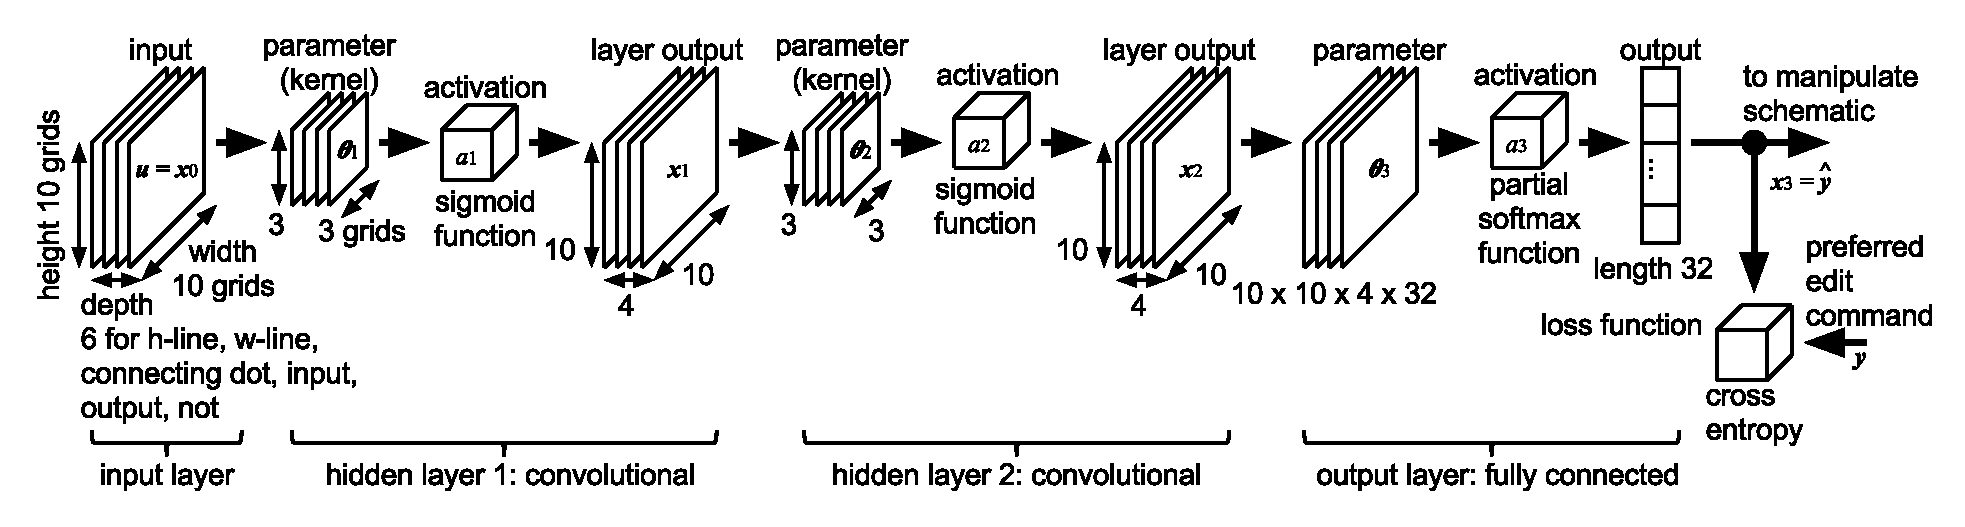
\includegraphics[width=\hsize]{fig/layers_06.eps}
   \caption{a layer structure of the neural network}
   \label{fig:layers}
  \end{minipage}
 \end{center}
\end{figure*}

Figure \ref{fig:encode} (e) shows how to encode schematic edit commands.
As can be seen also in Fig.\ \ref{fig:nn_schem},
a command consists of following 4 elements:
\begin{itemize}
\item command type, either move-x or move-y
\item origin-x
\item origin-y
\item destination
\end{itemize}
Move-x means to move a circuit element horizontally,
as shown in Fig. \ref{fig:nn_schem} (b').
Move-y is for vertically moving, as shown in
Fig.\ \ref{fig:nn_schem} (a') and (c').
In Fig.\ \ref{fig:nn_schem} (a'), 
For the command `move-x (2, 1) to 4' appearing
in Fig.\ \ref{fig:nn_schem} (a'),
origin-x, origin-y and destination are 2, 1 and 4 respectively.
It can be interpreted as to horizontally move an element
at the coordinate (2, 1) to (2, 4).
Each edit command element is encoded in one-hot form,
in which only one value is 1 and the others are 0 in a vector,
as shown in Fig.\ \ref{fig:encode} (e).
Move-x is encoded to the vector $[1.0, 0.0]$, 
while move-y is encoded to the vector $[0.0, 0.1]$. 
Origin-x is encoded as follows;
\begin{itemize}
\item $[1.0, 0.0, 0.0, 0.0, \cdots]$ for 0,
\item $[0.0, 1.0, 0.0, 0.0, \cdots]$ for 1, 
\item $[0.0, 0.0, 1.0, 0.0, \cdots]$ for 2,
\end{itemize}
and so on.
For origin-x, the length of the one-hot vector is the width of
the schematic diagram.
The origin-y is also encoded to one-hot vector which length is
height of the schematic diagram.
As well, destination is one-hot vector which length is
maximum value of width and height of the schematic diagram.
Output vector of the neural network is obtained
by concatenating those 4 one-hot vectors.
Those edit commands do not change semantics of schematics.

\section{Experimental Condition}

A neural network structure shown in Fig.\ \ref{fig:layers} is
applied in this work.
It has an input layer, 2 hidden layers and an output layer.
The input layer has width of 10, height of 10,
depth of 6 for horizontal nets, vertical nets, connecting dots, input ports,
output ports and not gates.

\begin{figure}[!tb]
 \begin{center}
  \begin{minipage}{\hsize}
   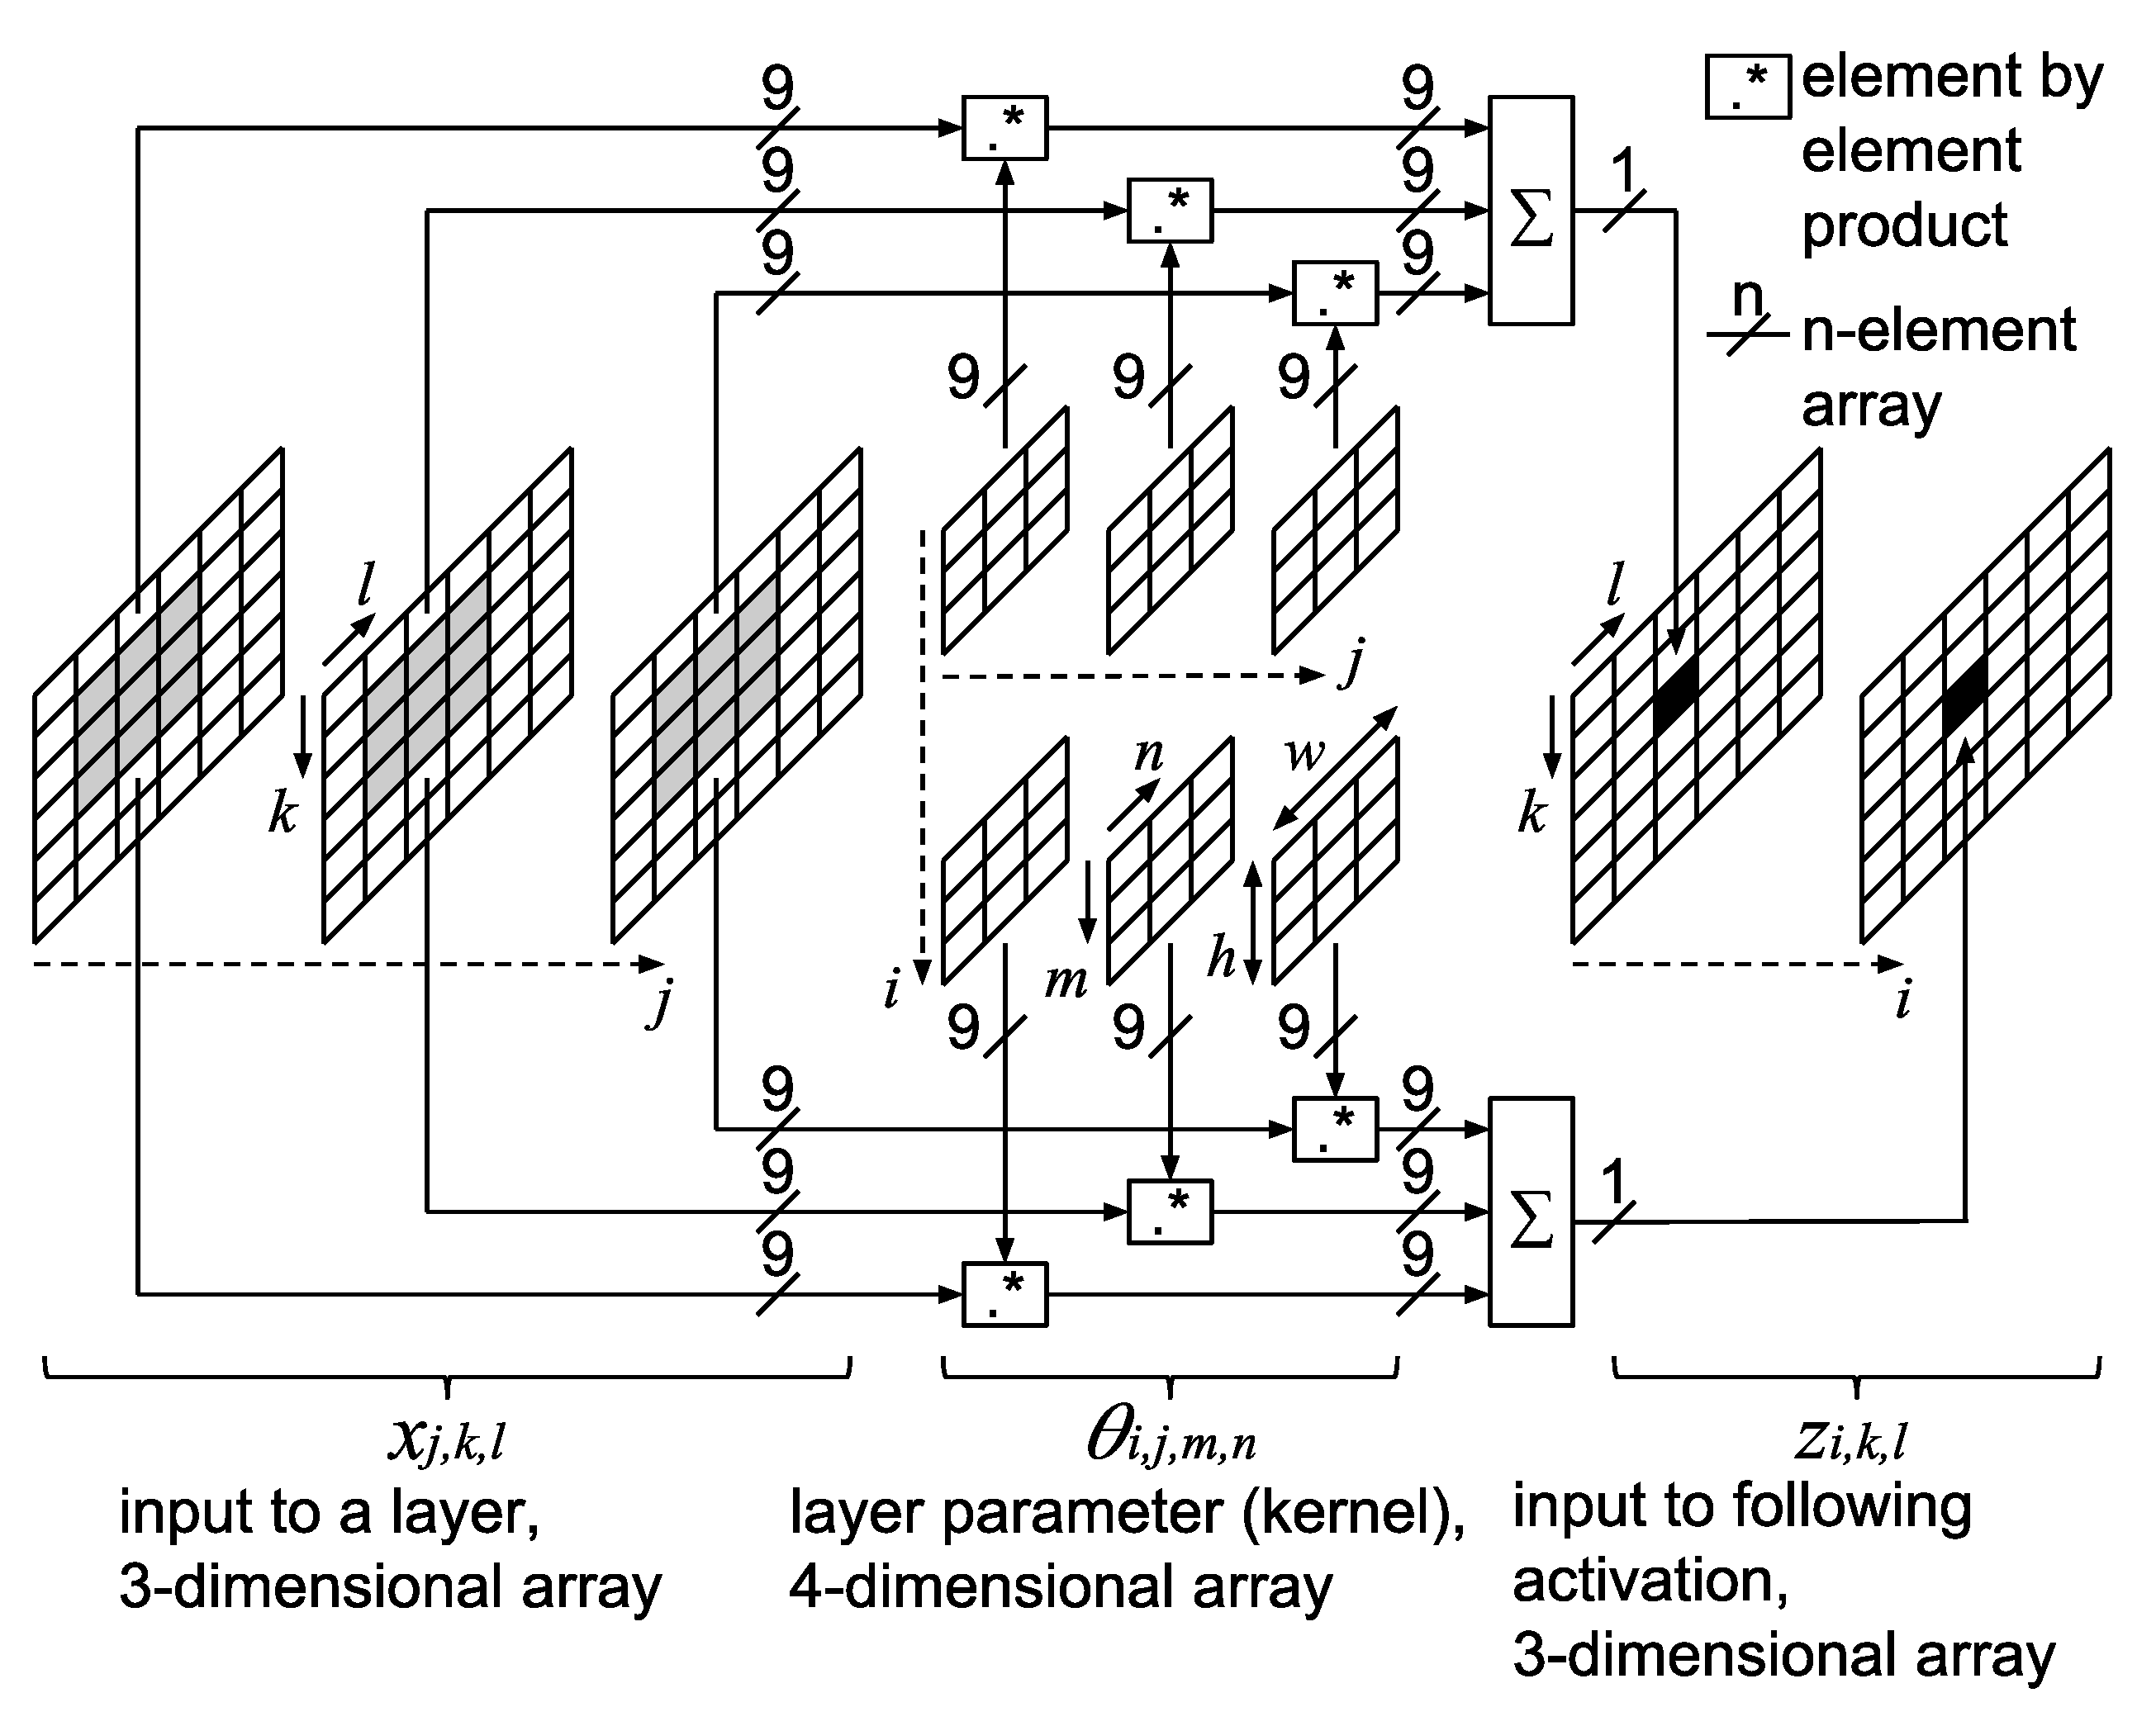
\includegraphics[width=\hsize]{fig/layer_convolutional_03.eps}
   \caption{convolutional layer}
   \label{fig:layer_convolutional}
  \end{minipage}
 \end{center}
\end{figure}

{\it Convolutional layer} described in \cite{mit} is applied
to hidden layers 1 and 2
to extract local characteristics of layer input.
Figure \ref{fig:layer_convolutional} shows the weight function
$f({\bf x}, {\bm \theta})$ of the convolutional layer,
where inputs to and outputs from $f$ are interpreted as
3-dimensional arrays which are denoted as $x_{j,k,l}$ for input,
$z_{i,k,l}$ for output with 3 subscripts.
With 4-dimensional parameter $\theta_{i,j,m,n}$,
the output $z_{i,k,l}$ is calculated as;
\begin{eqnarray}
z_{i,k,l} = \sum_{j}\sum^{h-1}_{m=0}\sum^{w-1}_{n=0}
\theta_{i,j,m,n}\,
 x_{j,k - \lfloor w/2 \rfloor + m,l - \lfloor h/2 \rfloor + n}
\end{eqnarray}
where $w$ and $h$ are width and height of the parameter array
as shown in Fig. \ref{fig:layer_convolutional}.

\begin{figure}[!tb]
 \begin{center}
  \begin{minipage}{\hsize}
   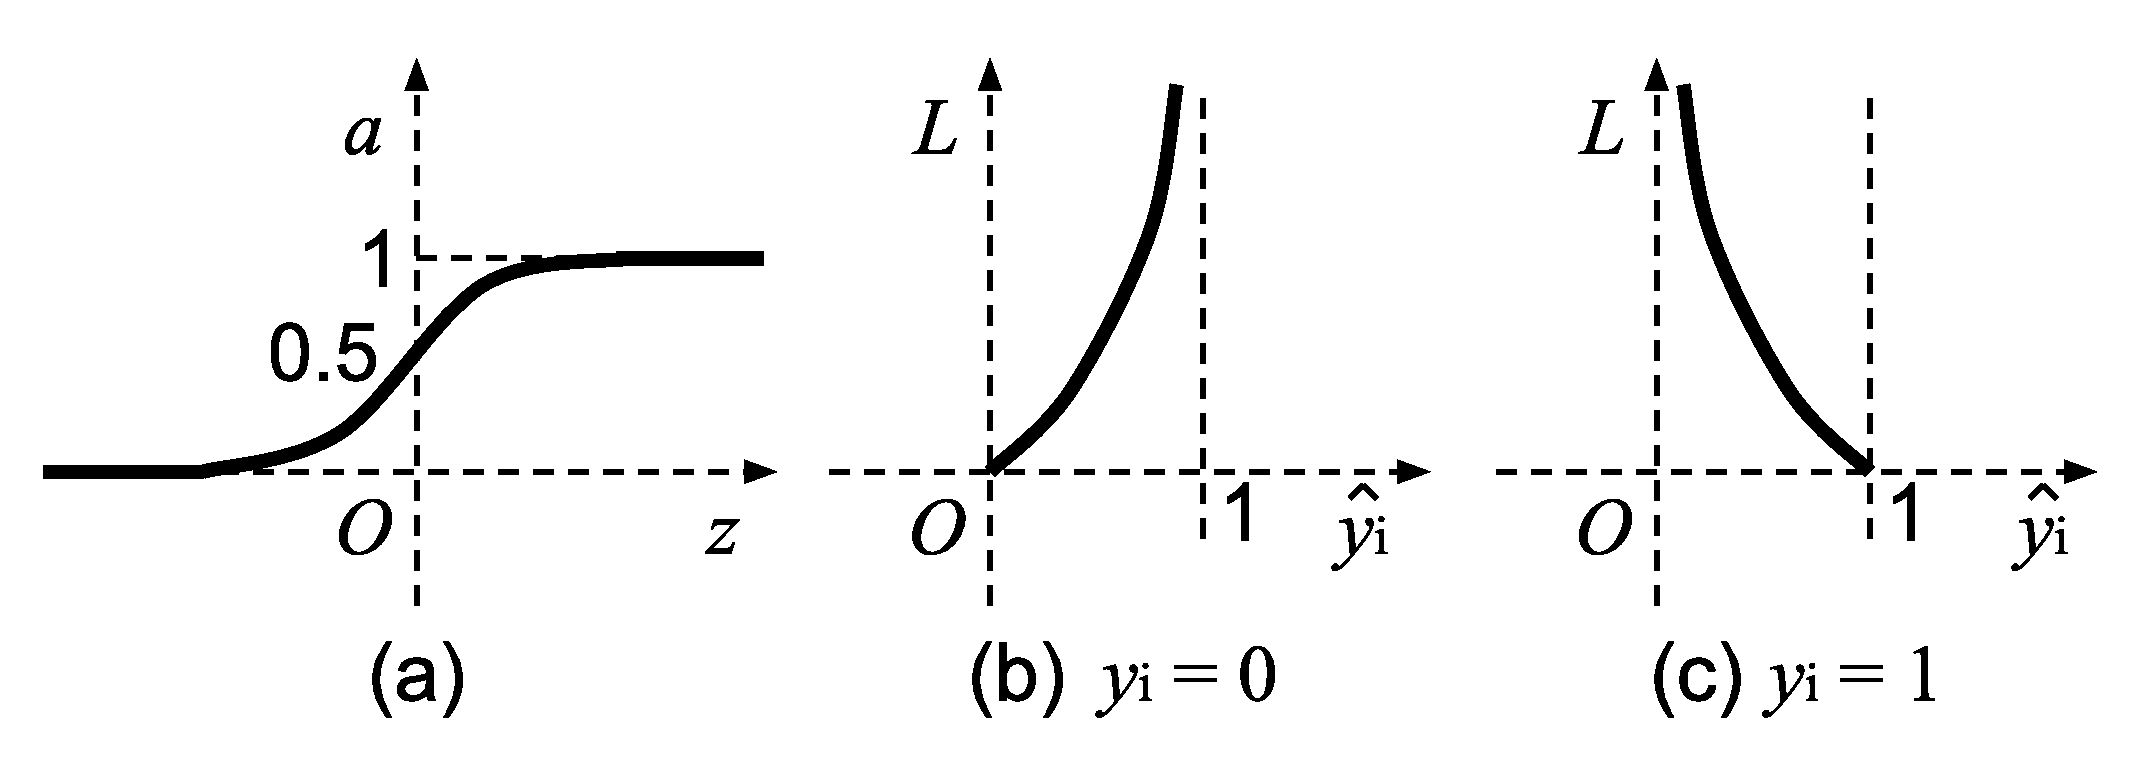
\includegraphics[width=\hsize]{fig/curves_03.eps}
   \caption{(a) sigmoid function
    (b) cross entropy function for $y_i = 0$ (c) for $y_i = 1$}
   \label{fig:curves}
  \end{minipage}
 \end{center}
\end{figure}

For activation function $a({\bf z})$ of hidden layers 1 and 2,
following sigmoid function is used:
\begin{eqnarray}
a(z_i) = \frac{1}{1+\exp(-z_i)}
\end{eqnarray}
Figure \ref{fig:curves} (a) shows the sigmoid function,
which clips large negative values to 0, large positive values to 1,
to digitize outputs of weight function.

For the output layer, {\it fully connected layer} is adopted.
It extracts global characteristics of the layer input
which is locally extracted one in an adjacent preceding layer.
Input and output of weight function 
$f({\bf x}, {\bm \theta})$
are regarded as 1-dimensional vectors,
so the formula looks like multiplication of a vector and a matrix as follows:
\begin{eqnarray}
z_i = \sum_{j} \theta_{i,j}\, x_{j}
\end{eqnarray}

\begin{figure}[!tp]
 \begin{center}
  \begin{minipage}{\hsize}
   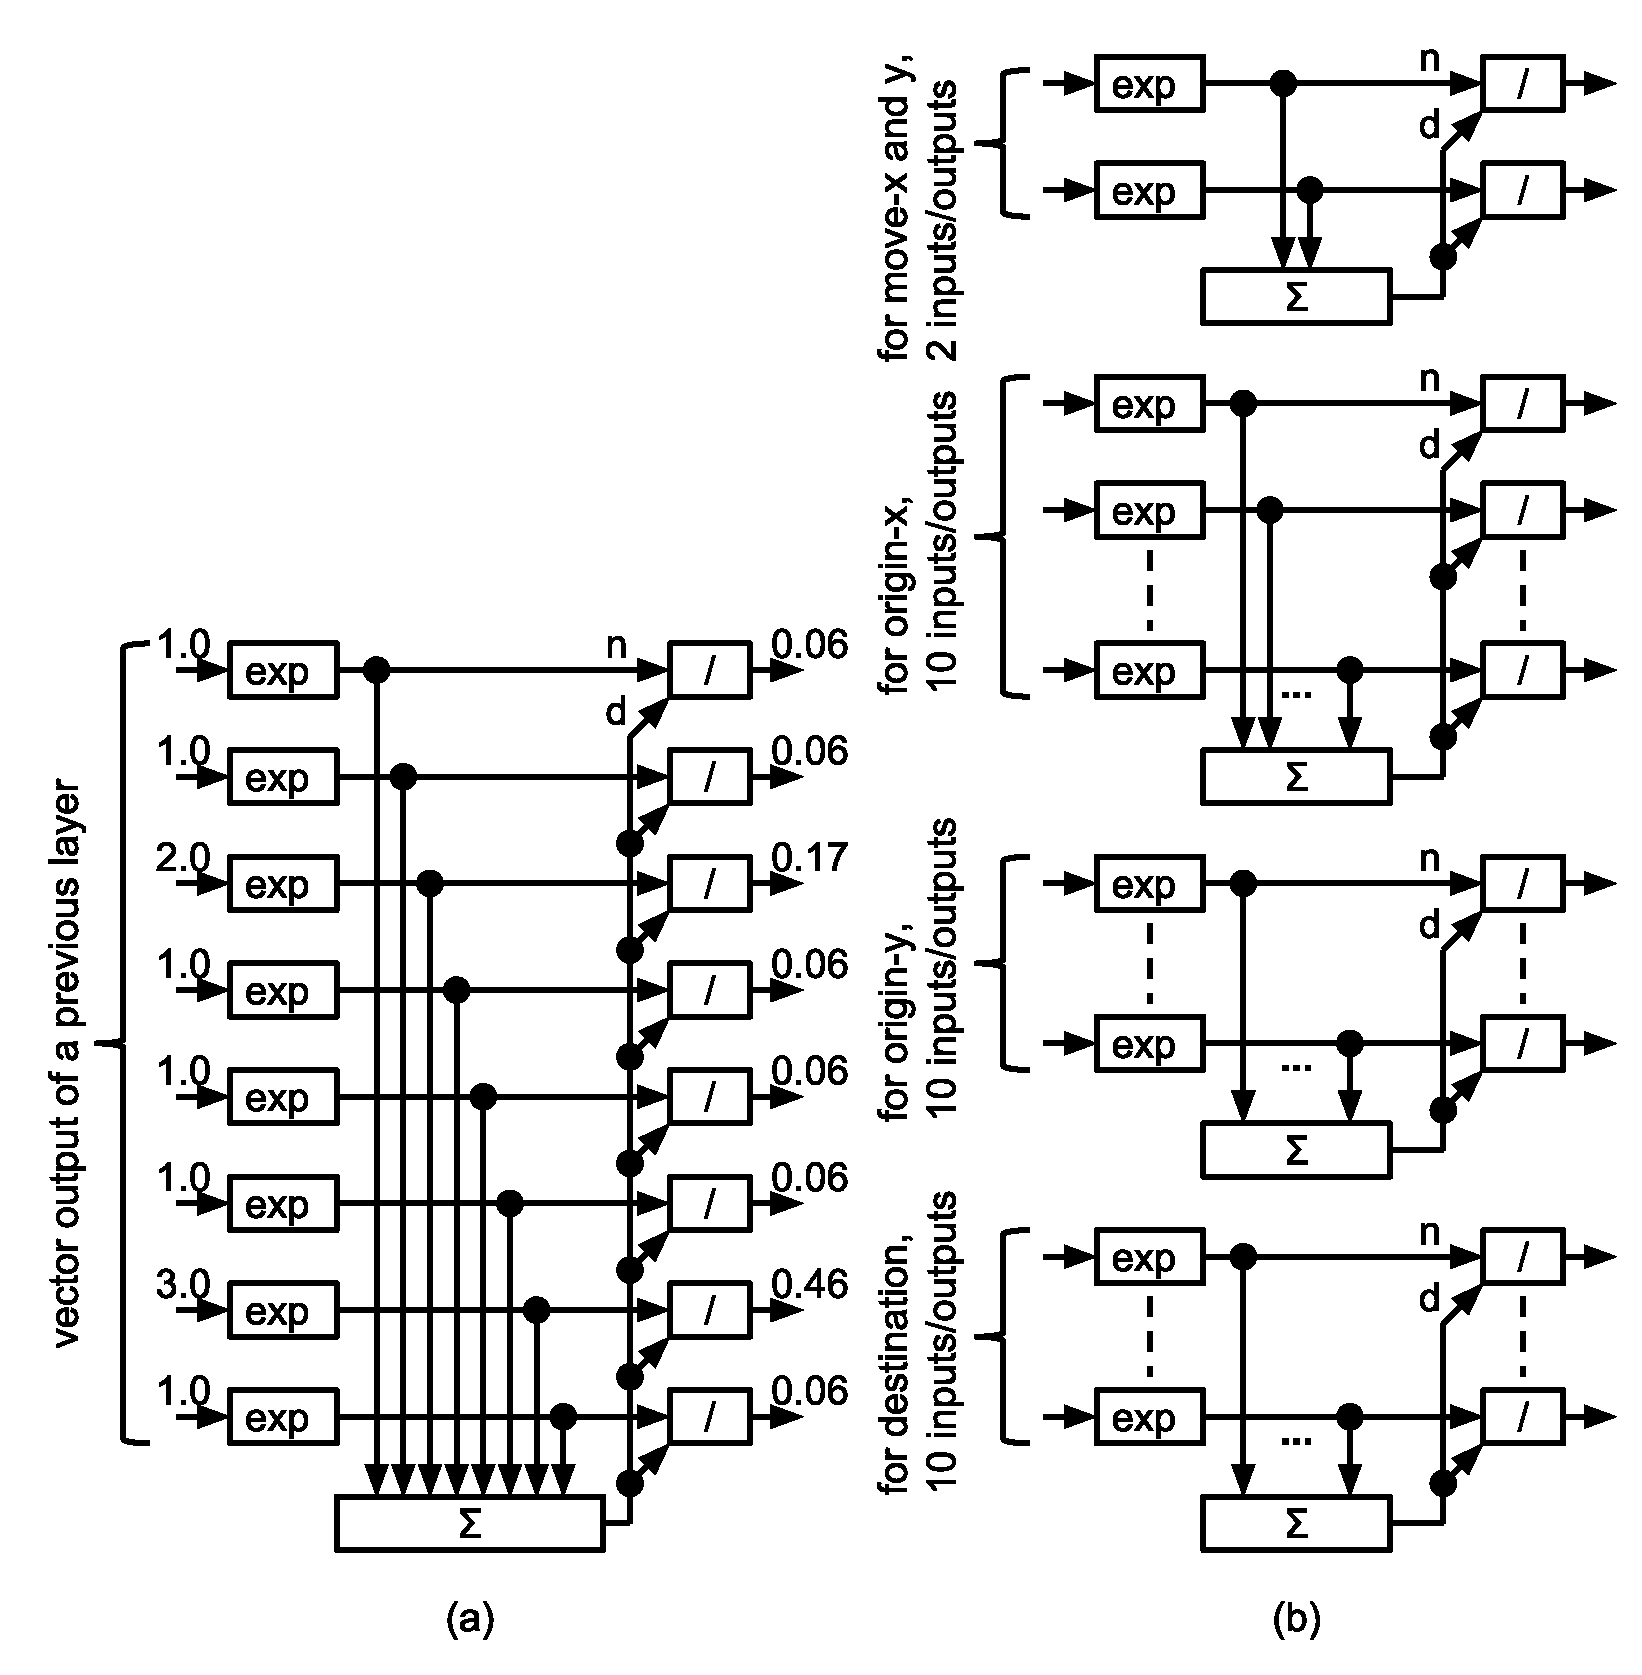
\includegraphics[width=\hsize]{fig/partial_softmax_05.eps}
   \caption{(a) conventional softmax, (b) partial softmax used in this paper.}
   \label{fig:partial_softmax}
  \end{minipage}
 \end{center}
\end{figure}

Softmax function is used for activation of the output layer.
It is formally described as:
\begin{eqnarray}
a({\bf z}) = \frac{\exp(z_i)}{\sum_j \exp(z_j)}
\end{eqnarray}
It emphasizes a maximum value in its input vector
as shown in Fig.\ \ref{fig:partial_softmax} (a)
which is a graphical expression of the softmax function.
Softmax function is used to pickup one maximum element of a vector
if the vector has intrinsically one-hot form.
For our application where an 32-length output vector could be split
into 4 fragments which sizes are
2 (for command type), 10 (for origin-x), 10 (for origin-y)
and 10 (for destination)
and each fragment should be intepreted as a one-hot form,
it is not appropriate to emphasize only one element among the 32 elements.
Each fragment should be applied to softmax function
as shown in Fig.\ \ref{fig:partial_softmax} (b).
Let us call it as {\it partial softmax} in this paper.
Softmax function poses a stronger restriction to its output
and contributes to faster learning convergence than sigmoid function,
while sigmoid function could be applied to the output layer activation.

For loss function
$L(\hat{\bf y}({\bf u},{\bm \theta}_1,\cdots,{\bm \theta}_N),{\bf y})$,
{\it cross entropy function} shown in Fig.\ \ref{fig:curves} (b) and (c)
is used, which is formally denoted as;
\begin{eqnarray}
L(\hat{\bf y},{\bf y})
= \sum_i \left[ - y_i \log \hat{y_i} - (1-y_i) \log (1-\hat{y_i}) \right]
\end{eqnarray}
which sums up $y_i$ and $\hat{y_i}$ applied to the function.
$y_i$ and $\hat{y_i}$ are elements of a target vector ${\bf y}$ and
the corresponding output vector $\hat{\bf y}$.
For the target value $y_i = 0$,
the cross entropy function forms the curve
shown in Fig.\ \ref{fig:curves} (b).
When an target value $y_i = 0$, in other words,
the output value $\hat{y_i}$ matches to $y_i$,
$L$ is calculated as 0, no error.
The farther $\hat{y_i}$ is from $y_i$, the larger $L$ becomes.
Even though the $L$ is not defined in a range
$\hat{y_i} \le 0, 1 \le \hat{y_i}$,
it is applicable because a preceding activation function
restricts $\hat{y}_i$ in a range $0 < \hat{y}_i < 1$.
While Euclidean distance
$L(\hat{\bf y}, {\bf y}) = \sum_i (\hat{y}_i - y_i)^2$
could be used as a kind of the simplest loss functions,
it less significantly evaluates the error between $\hat{\bf y}$ and ${\bf y}$
and results in a slower convergence of learning.

\begin{figure}[!tp]
  \begin{minipage}{\hsize}
 \begin{center}
   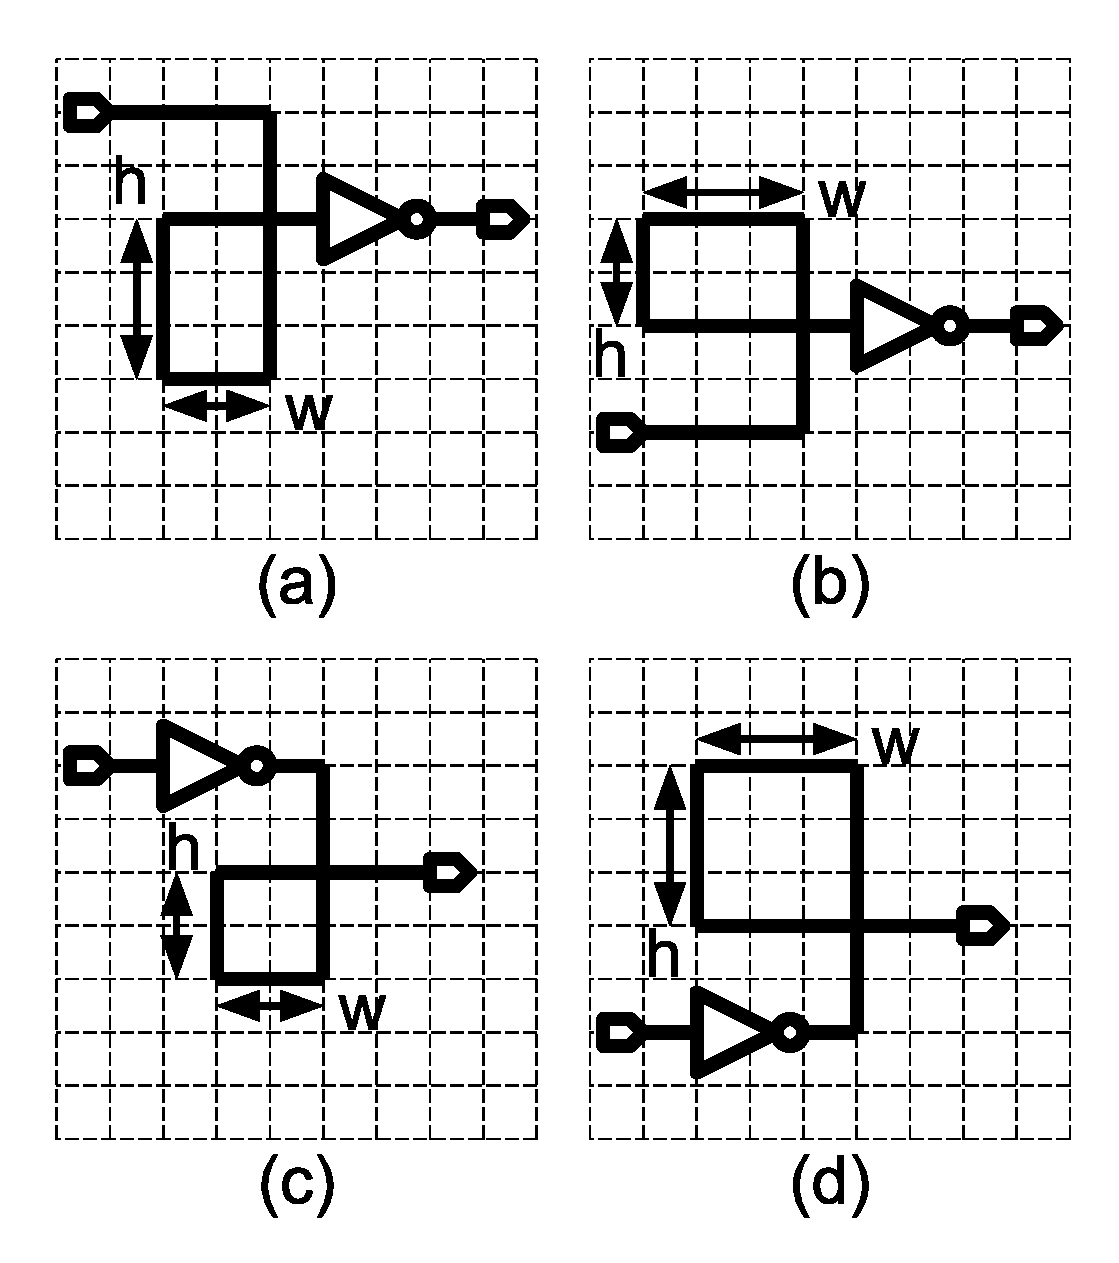
\includegraphics[width=0.7\hsize]{fig/training_data_02.eps}
   \caption{training data}
   \label{fig:training_data}
 \end{center}
  \end{minipage}
\end{figure}

Schematics shown in Fig.\ \ref{fig:training_data} are used for data set
in this experiments.
Each one consists of one input port, one not gate and one output port.
It also contains an unnecessary ring which will be removed
by the edit commands generated by the trained neural network.
Each schematic diagram of Fig.\ \ref{fig:training_data} (a), (b), (c) and (d)
has 9 variations with
$w$ of 2, 3 and 4, for the widht of the ring,
$h$ of 2, 3 and 4, for the height of the ring.
Then, there are 9 variations for the size of the ring.
Thus, $9 \times 4 = 36$ different schematic patterns are introduced.
Field size of those schematics is 10 grids $\times$ 10 grids.
Since the schematic field has margin around the circuitry,
the schematics can be placed various position on schematic field.
Finally, several schematic edit steps are introduced
to achieve a clean schematic diagram.
The total number of schematic-edit-command pairs amounts up to about 1000,
which the data set consists of.

The following hyper-parameters are used:
0.1 for learning rate $\epsilon$,
16 for minibatch size $M$,
$10^{-4}$ for weight decay $\lambda$ and 10000 of traning iteration.
The program is written in Java and Clojure which is
a dialect of Lisp running on Java Virtual Machine.

\section{Result}

\begin{figure}[!tp]
 \begin{center}
  \begin{minipage}{\hsize}
   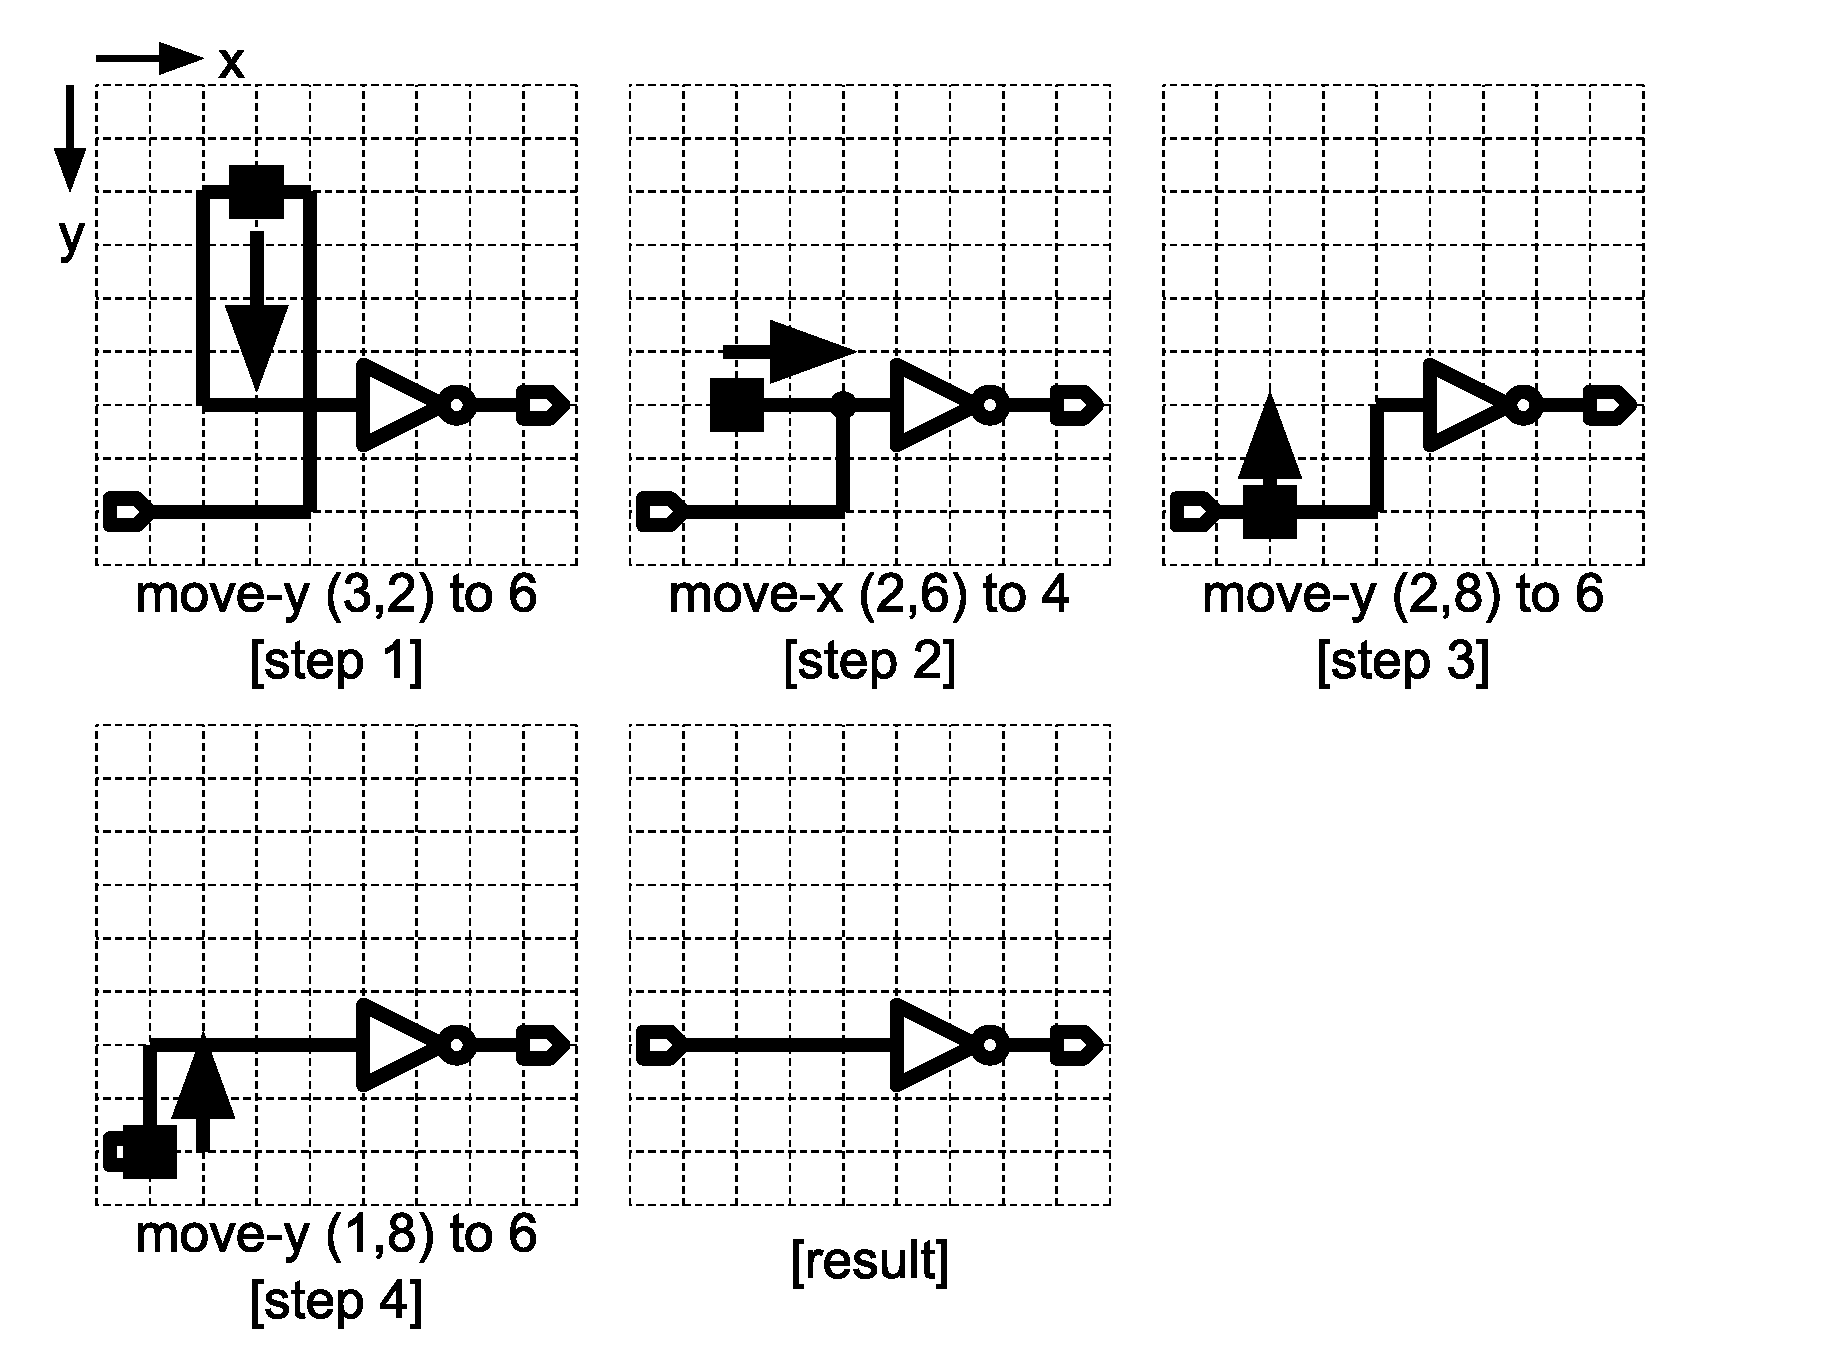
\includegraphics[width=\hsize]{fig/edit_steps_03.eps}
   \caption{Steps to aestheticize a schematic diagram
            generated by a trained neural network.}
   \label{fig:edit_steps}
  \end{minipage}
 \end{center}
\end{figure}

Figure \ref{fig:edit_steps} shows a sequence of schematic edit steps
automatically generated from the trained neural network.
36 schematic patterns shown in Fig.\ \ref{fig:training_data}
were split into 12 patterns for training data set
and the remaining 24 patterns,
then a schematic diagram was picked up
from 24 patterns to test the learning result
and to generate the edit sequence.
The neural network was trained with vectors
orinating only from the 12 patterns for training.
In Fig. \ref{fig:edit_steps}, filled square shows the origin-x and y
for each step.
At step 1, the top net of the unnecessary ring is grabbed and moved lower
to remove the ring.
At step 2, the edge of salient net is grabbed,
and moved to the adjacent cross point.
At step 3, the net connected to the input port is grabbed.
Finally, at step 4, the input port is moved upward
and a clean schematic diagram is achived.
The neural network succeeded in cleaning up a schematic diagram
which the network has never experienced.
The running time of this schematic edit command generation
is less than 1 second.

\begin{figure}[!tp]
 \begin{center}
  \begin{minipage}{\hsize}
   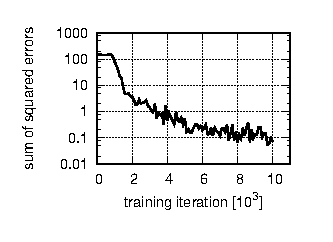
\includegraphics[width=\hsize]{fig/errors.eps}
   \caption{Convergence of learning.}
   \label{fig:errors}
  \end{minipage}
 \end{center}
\end{figure}

Figure \ref{fig:errors} shows an error observed in learning phase.
The horizontal axes is traning iteration up to 10000.
The vertical axes is the sum of squared errors between
output vectors $\hat{\bf y}_i$ and target vectors ${\bf y}_i$
calculated as follows;
\begin{eqnarray}
\sum_i||\hat{\bf y}_i - {\bf y}_i||^2
\end{eqnarray}
where the expression with double bars $||\hat{\bf y} - {\bf y}||^2$ 
means squared Euclidean distance between 2 vectors as follows:
\begin{eqnarray}
||\hat{\bf y} - {\bf y}||^2 =
\sum_j(\hat{y}_j - y_j)^2
\end{eqnarray}
16 pairs of output vector $\hat{\bf y}_i$ and target vector ${\bf y}_i$
were picked up from the training data set to confirm the convergence.
The curve gets close to 0, and convergence of learning can be seen there.
Due to the decay weight $\lambda$ to avoid overfitting,
the curve keeps a value slightly more than 0.
It took 60 seconds to finish the 10000 training iterations,
on an Intel Core i5-4300U CPU 1.9\,GHz.

\begin{figure}[!tp]
 \begin{center}
  \begin{minipage}{\hsize}
   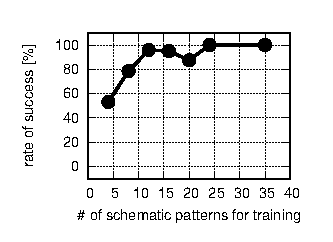
\includegraphics[width=\hsize]{fig/test_data.eps}
   \caption{Success rate of making schematics aesthetic.}
   \label{fig:test_data}
  \end{minipage}
 \end{center}
\end{figure}

This experiment has been performed, varing the amount of training data set.
Figure \ref{fig:test_data} shows the result.
The horizontal axes shows the number of schematic patterns
used for traninig data set picked up from 36 patterns
shown in Fig.\ \ref{fig:training_data}.
Also in this experiment,
the training data set is separated from schematic patterns
used for test of learning performance.
The vertical axes shows the rate of success.
In this result, {\it success} means that a clean schematic diagram,
which looks like the final result in Fig.\ \ref{fig:edit_steps},
with no overcrossing or unnecessary corner is achived.
Even when trained with only 4 schematic patterns,
the neural network could clean up about 53\% of schematics
in the $36 - 4 = 32$ schematics.
When trained with 12 patterns,
which corresponds to one third of all 36 schematic patterns,
the success rate 95\% was achieved.
When trained with 24 patterns,
which corresponds to two thirds of all schematic patterns,
the success rate reached to 100\%.

\section{Conclusions}

An novel way to achieve aesthetic schematic is proposed.
Deep neural network is used, and it learns how to edit schematic
from edit history obtained from human.
The trained neural network cleans up unnecessary part of given schematics,
which the neural network has not experienced.
Even the neural network is short of traning data,
it can clean up unknown schematics to a certain extent.
With enough training data,
the trained neural network can clean up almost of schematic.

%this is how to do an unnumbered subsection 
%\section*{\sc Acknowledgements}
%This article was written by referring to {\em ``Author's guide --
%Preparation of Papers in Two-Column Format for VLSI Symposia on
%Technology and Circuits''}, the {\em ``Preparation of Papers in
%Two-Column Format for the Proceedings of the 32nd ACM/IEEE Design
%Automation Conference''} written by Ann Burgmeyer, IEEE and {\em ``the
%template for producing IEEE-format articles using \LaTeX''}, written by
%Matthew Ward, Worcester Polytechnic Institute.

\begin{thebibliography}{99}
\footnotesize

\bibitem{ph}
D. A. Patterson, and J. L. Hennessy,
{\em Computer Organization and Design MIPS Edition:
 The Herdware/Software Interface,}
Morgan Kaufmann, 2013.

\bibitem{nauts}
C. Nauts,
``Creating a nice-looking schematic from its netlist description,''
in {\em Proc. Euro ASIC}, Mar. 1992.

\bibitem{anshul}
A. Kumar, A, Arya, V. V. Swaminathan, and A. Misra,
``Automatic Generation of Digital System Schematic Diagrams,''
{\em IEEE Design \& Test of Computers,}
vol. 3, pp. 58--65, 1986.

\bibitem{fiduccia}
C. M. Fiduccia, and R. M. Mattheyses,
``A Linear-Time Heuristic for Improving Network Partitions,''
in {\em Proc. IEEE/ACM Design Automation Conference(DAC),}
Jun. 1982.

\bibitem{chun}
R. K. Chun, K.-J. Chang, and L. P. McNamee,
``VISION: VHDL Induced Schematic Imaging on Net-Lists,''
in {\em Proc. IEEE/ACM Design Automation Conference(DAC),}
Jun. 1987.

\bibitem{green}
L. D. Green, and J. Andersen,
``Automated generation of analog schematic diagrams,''
in {\em Proc. IEEE International Symposium on Circuits and Systems(ISCAS),}
May. 1990.

\bibitem{tsung}
T. D. Lee, and L. Pl. McNamee,
``Aesthetic Routing for Transistor Schematics,''
in {\em Proc. IEEE/ACM International Conference
 on Computer-Aided Design(ICCAD),}
Nov. 1992.

\bibitem{bogdan}
B. G. Arsintescu,
``A Method for Analog Circuits Visualization,''
in {\em Proc. International Conference on Computer Design (ICCD),}
Oct. 1996.

\bibitem{fan}
F. Lin, and K.-T. Cheng,
``An Artificial Neural Network Approach for Screening Test Escapes,''
in {\em Proc. Asia and South Pacific Design Automation Conference (ASP-DAC),}
Jan. 2017.

\bibitem{sourav}
S. Das, J. R. Doppa, D. H. Kim. P. P. Pande, and K. Chakrabarty,
``Optimizing 3D NoC design for energy efficiency:
 A machine learning approach,''
in {\em Proc. IEEE/ACM International Conference on
 Computer-Aided Design (ICCAD),}
Nov. 2015.

\bibitem{nips}
A. Krezhevsky, I. Sutskever, and G. E. Hinton,
``ImageNet Classification with Deep Convolutional Neural Networks,’’
in {\em Proc. Annual Conference on Neural Information Processing Systems (NIPS)},
Dec. 2012.


\bibitem{alphago}
D. Silver, A. Huang, C. J. Maddison, A. Guez, L. Sifre, G. van den Driessche,
J. Schrittwieser, I. Antonoglou, V. Panneershelvam, M. Lanctot, S. Dieleman,
D. Grewe, J. Nham, N. Kalchbrenner, I. Sutskever, T. Lillicrap, M. Leach,
K. Kavukcuoglu, T. Graepel, and D. Hassabis,
``Mastering The Game of Go with Deep Neural Networks And Tree Search,’’
{\em Nature,} vol. 529, pp. 484--489, 2016.

\bibitem{mit}
I. Goodfellow, Y. Bengio, and A. Courville,
{\em Deep Learning (Adaptive Computation and Machine Learning),}
The MIT Press, 2016. 

\end{thebibliography}
\end{document}
